\documentclass[11pt]{article}
%
\usepackage[parfill]{parskip}
\usepackage{amsmath}   
\usepackage{amsthm}
\usepackage{amssymb} 
\usepackage{calc}
\usepackage{centernot}
\usepackage{ifthen}
\usepackage{graphicx}
\usepackage{enumerate}
\usepackage[mathscr]{eucal}



%MATH FORMATTING
\renewcommand\bf[1]{\ensuremath{\mathbf{#1}}}
\renewcommand\cal[1]{\ensuremath{\mathcal{#1}}}
\newcommand\bb[1]{\ensuremath{\mathbb{#1}}}
\newcommand\call{\stackrel{\text{\tiny call}}{=}}
\newcommand\thru[2]{\ensuremath{#1,\ldots,#2}}
\newcommand\rank[1]{\ensuremath{\text{Rank}(#1)}}
\newcommand\tboxed[1]{\boxed{\text{#1}}}
%\renewcommand\and{\ensuremath{\;\;\;\;\;\;\text{and}\;\;\;\;\;\;} }
\newcommand\where{\ensuremath{\;\;\;\text{where}\;\;\;}}
\newcommand\suchthat{\ensuremath{\;\;\;\text{s.t.}\;\;\;}}
\newcommand\nn{\nonumber}
\newcommand\mcal[1]{\ensuremath{\mathcal{#1}}}
\newcommand\from[1]{\ensuremath{_{#1}}}
\renewcommand\to[1]{\ensuremath{^{#1}}}
\renewcommand\eqref[1]{Eq. (\ref{#1})}
\newcommand\pref[1]{(\ref{#1})}
\newcommand\upa{\ensuremath{\uparrow}}
\newcommand\dna{\ensuremath{\downarrow}}
\renewcommand\deg{\ensuremath{^\circ}}


%GREEK
\newcommand\bs[1]{\boldsymbol{#1}}
\newcommand\Om{\ensuremath{\Omega} }
\newcommand\om{\ensuremath{\omega}}
\newcommand\ep{\epsilon}
\newcommand\g{\gamma}
\newcommand\G{\Gamma}
\newcommand\D{\Delta}
\renewcommand\r{\rho}
\newcommand\m{\mu}
\newcommand\al{\alpha}
\newcommand\la{\ensuremath{\lambda} }


%FUNCTIONS
 \newcommand\csch{\text{csch}}
 \newcommand\inv[1]{\ensuremath{#1^{-1}}}
 \newcommand\vol[1]{\text{vol}(#1)} 
 \newcommand\ceiling[1]{\ensuremath{\left  \lceil #1 \right \rceil}}
 \newcommand\ceil[1]{\ensuremath{\left  \lceil #1 \right \rceil}}
 \newcommand\floor[1]{\ensuremath{ \left \lfloor #1 \right \rfloor}}
  \newcommand\sign[1]{\ensuremath{\text{sign}(#1)}}
 
 %LOGIC
 \newcommand\notimplies{\centernot\implies}

%%SET THEORY%%
\newcommand\seq{\ensuremath{\subseteq}}
\newcommand\nin{\ensuremath{\notin}}
\newcommand\union{\ensuremath{\cup}}
\newcommand\Union{\ensuremath{\bigcup}}
\newcommand\intersection{\ensuremath{\cap}}
\newcommand\intersect{\ensuremath{\cap}}
\newcommand\Intersection{\ensuremath{\bigcap}}
\newcommand\Intersect{\ensuremath{\bigcap}}
\newcommand\es{\ensuremath{\emptyset}}
 
%%ALGEBRA%%
\newcommand\leqc{\trianglelefteq}
 
 %%ANALYSIS
 \newcommand\hs{\ensuremath{\cal{H}} }
 \newcommand\lp[1]{\ensuremath{ {L^#1(\bb{R}^d)}}}
  \newcommand\LpRd{\ensuremath{ {L^P(\bb{R}^d)}}}
  \newcommand\Lp{\ensuremath{ {L^P}}}  
 \newcommand\Rd{\ensuremath{ {\bb{R}^d} }}
 \newcommand\R{\ensuremath{\bb{R}}}
  \newcommand\Q{\ensuremath{\bb{Q}} }
 \newcommand\Z{\ensuremath{\bb{Z}}}
 \newcommand\C{\ensuremath{\bb{C}}}
 \newcommand\N{\ensuremath{\bb{N}}}
 \newcommand\T{\ensuremath{\bb{T}}}
 \newcommand\Td{\ensuremath{ \bb{T}^d}}
 \newcommand\sa{$\sigma$\text{--algebra}}
 \newcommand\order[1]{\ensuremath{\cal{O}(#1)}}

%%PROBABILITY
 \newcommand\sigmafield{\ensuremath{\sigma\text{--field}}}
  \newcommand\lsystem{\ensuremath{\lambda\text{--system}}}
  \newcommand\psystem{\ensuremath{\pi \text{--system}}}
 
 %%PHYSICAL CONSTANTS
 \newcommand\h{\ensuremath{\hbar}}
 \newcommand\hb{\ensuremath{\hbar}}
 
 %%PHYSICS%%
 \newcommand\pb[2]{\ensuremath{ \left [#1, #2 \right ]_{PB}}} 

%% CALC/QUANTUM %%
\newcommand\abs[1]{\ensuremath{\left\vert #1\right \vert}}
\newcommand\Bigabs[1]{\ensuremath{\Bigl\vert #1 \Bigr\vert}}
\newcommand\biggabs[1]{\ensuremath{\biggl\vert #1 \biggr\vert}}

\newcommand\norm[1]{\ensuremath{\lvert \lvert  #1 \rvert \rvert }} 
\newcommand\Tr[1]{\ensuremath{\text{Tr}(#1) }} 
\newcommand\Bignorm[1]{\ensuremath{\Bigl\lvert \Bigl\lvert  #1 \Bigr\rvert \Bigr\rvert }} 

\newcommand\ip[1]{\ensuremath{\left\langle#1\right\rangle}}

\newcommand\avg[2][1]{
	\ifthenelse{\equal{#1}{1}}{\ensuremath{\left \langle#2\right \rangle }}{}
	\ifthenelse{\equal{#1}{2}}{\ensuremath{\left \langle#2^2\right \rangle }}{}
	\ifthenelse{\equal{#1}{3}}{\ensuremath{\left \langle#2\right \rangle ^2}}{}}

\newcommand\derv[3][1]{
	\ifthenelse{\equal{#1}{1}}{\ensuremath{\frac{d#2}{d#3}}}{ 
		\ensuremath{\frac{d^#1 #2}{d#3^#1}}
	}
}

\newcommand\totalderv[2]{\ensuremath{\frac{\text{d}#1}{\text{d}#2}}}

\newcommand\prtl[3][1]{	\ifthenelse{\equal{#1}{1}}{\ensuremath{\frac{\partial#2}{\partial#3}}}{}
	\ifthenelse{\equal{#1}{2}}{\ensuremath{\frac{\partial^2#2}{\partial#3^2}}}{}}
	
\newcommand\db{\ensuremath{\mathchar'26\mkern-12mu d}} 
	
\newcommand\bra[1]{\ensuremath{\langle#1\vert}}
 \newcommand\ket[1]{\ensuremath{\vert #1 \rangle}} 
 \newcommand\bk[2]{\ensuremath{\langle#1\vert#2\rangle}}
\newcommand\re[1]{\ensuremath{\text{Re}(#1)}}
\newcommand\im[1]{\ensuremath{\text{Im}(#1)}}

\newcommand\intall[2][x]{\int_{-\infty}^\infty #2 d #1}	


\newcommand\mathc{\ensuremath{\textbf{C}}}
\newcommand\mathr{\ensuremath{\textbf{R}}}
\newcommand\res{\ensuremath{\text{Res}}}
\newcommand\confeq{\ensuremath{\stackrel{\sim}{\rightarrow}}}	


%MATRIX%
\newcommand\qmatrix[9]{
 \left( \begin{array}{ccc}
 #1&#2&#3\\
 #4&#5&#6\\
 #7&#8&#9
 \end{array} \right)}
 
 \newcommand\sqmatrix[4]{
 \left( \begin{array}{cc}
 #1&#2\\
 #3&#4
  \end{array} \right)}

 \newcommand\matTWO[4]{
 \left( \begin{array}{cc}
 #1&#2\\
 #3&#4
  \end{array} \right)}

 \newcommand\matTHREE[9]{
 \left( \begin{array}{ccc}
 #1&#2&#3\\
 #4&#5&#6\\
 #7&#8&#9
  \end{array} \right)}
 

 \newcommand\mat[2][cccccccccccccccccccccc]{
 \left[ \begin{array}{#1} 
 #2\\
 \end{array} \right]}

% \newcommand\det[2][rrrrrrrrrrrrrrrrrrrrrrrrrrrrrr]{
 %\left| \begin{array}{#1} 
 %#2\\
 %\end{array} \right|}

 \newcommand\qdet[9]{
 \left\vert \begin{array}{ccc}
 #1&#2&#3\\
 #4&#5&#6\\
 #7&#8&#9
 \end{array} \right\vert}

  \newcommand\sqdet[4]{
 \left\vert \begin{array}{cc}
 #1&#2\\
 #3&#4
  \end{array} \right\vert}
 
 \newcommand\qvec[3]{
  \left( \begin{array}{c}
 #1\\
 #2\\
 #3
  \end{array} \right)}

 \newcommand\sqvec[2]{
  \left( \begin{array}{c}
 #1\\
 #2
  \end{array} \right)}
  
  %MATLAB%
  \newcommand\tril[1]{\ensuremath{\text{tril}(#1)}}
  \newcommand\diag[1]{\ensuremath{\text{diag}(#1)}}

  
%DISPLAY  

%ENVIRONMENTS

\theoremstyle{plain}   \newtheorem{thm}{Theorem}
\renewcommand{\qedsymbol}{$\blacksquare$}
\theoremstyle{plain}   \newtheorem{lem}{Lemma}
\theoremstyle{definition}   \newtheorem*{defn}{Definition}
\theoremstyle{plain}   \newtheorem{post}{Postulate}
\theoremstyle{plain}   \newtheorem{prop}{Proposition}
\theoremstyle{plain}   \newtheorem{cor}{Corollary} 
\newcommand\problem[1]{\textbf{Problem #1}\\}
%{\renewcommand{\descriptionlabel}[1]{}

\newcommand\pspace[2][20]{$\hspace{#1pt}$~}
\usepackage{graphicx}
\usepackage{pxfonts}
\usepackage{algorithm}
\usepackage{algorithmic}
\usepackage{epstopdf}
\usepackage{fullpage}
\usepackage{epic}
\usepackage{eepic}

\begin{document}

\title{CS5625 Final Project Proposal}
\author{Michael Flashman \\ mtf53@cornell.edu \and Tianhe Zhang \\ tz249@cornell.edu\\}
\date{\today}
\maketitle


\section{Overview}
We propose a simple  game based the short play \textit{Act Without Words I}, by Samuel Becket.   
The setting for the game is sandy dessert under on blazing .  In the middle of this dessert  stands a palm tree, and a pile of perfect spheres.  The premise of the game is to launch these spheres off into the distance using the palm tree as an impromptu catapult.  See Figure 1.

\section{Technical Components}
The primary technical component of our game is the generation, animation, and rendering vegetation, specifically a  palm tree.  We will focus in particular on the procedural generation and accurate physical simulation.  Procedural generation begins with constructing a skeleton.  In the case of the palm tree, the skeleton is particularly simple. This skeleton provides a natural structure for simulating the physics of the tree.  (The hard work of the simulation will be left to a third party physics engine, such as jbullet.)  From the skeleton, we can generate a simple mesh for the tree using bone system methadology.  If time allows, we will implement normal or relief mapping for the bark on the trunk.

It may  be prohibitively slow to simulate the physics of every leaf.  To address this problem we follow the simulation optimization methodology described in [1].  That is,  we will only perform the simulation using a select number of leaves, and then interpolate to get the remaining leaf geometry.  

Finally, we will apply wind to our tree.  Many methods exist to create this effect, ranging from simple height-based vertex transformations, to more physically plausible procedural methods as in [2], to actually solving the full fluid equations.    The second one seems most interesting, but time constraints may force a simpler approach. 

%\begin{enumerate}
\section{Tentative Schedule}
\begin{itemize}
\item{Week 1: April 1 - April 7}

\begin{enumerate}
\item{Design a skeleton mesh procedurally for the palm tree rendering and physical simulation. - Michael, Tianhe }
\item{Explore a physics engine. - Michael}
\item{Try to connect to our base code. - Tianhe}
\item{If a feasible physics engine cannot be found, implement the physically based simulation such as collision detection. - Michael, Tianhe}
\end{enumerate}

\item{Week 2: April 8 - April 14}

\begin{enumerate}
\item{Tree model: build the basic tree mesh procedurally by using the skeleton mesh. - Michael}
\item{Terrain: build a basic terrain using subdivision surface. - Tianhe}

\end{enumerate}

\item{Week 3: April 15 - April 21}

\begin{enumerate}
\item{Learn the hair model described in [1] - Michael and Tianhe}
\item{Optimize leaves and fonds simulation by using the interpolation of leaves and fronds based on the hair model. - Michael, Tianhe}

\end{enumerate}

\item{Week 4: April 22 - April 28}

\begin{enumerate}
\item{Apply the physics simulation to the skeleton mesh. - Michael}
\item{Apply certain techniques to make the tree look nice. e.g. Normal mapping for the trunk. - Tianhe}
\end{enumerate}

\item{Week 5: April 29 - May 5}

\begin{enumerate}
\item{Game implementation: Shooting a rock to the desert.}
\item{Rock design - Michael}
\item{Target design - Tianhe}

\end{enumerate}

\item{Week 6: May 5 - May 11}

\begin{enumerate}
\item{Learn the wind animations for trees described in [2] - Michael, Tianhe}
\item{Implement wind simulation - Michael, Tianhe}
\item{Test and report - Michael, Tianhe}
\end{enumerate}

\end{itemize}

\begin{figure}[ht]
\centering
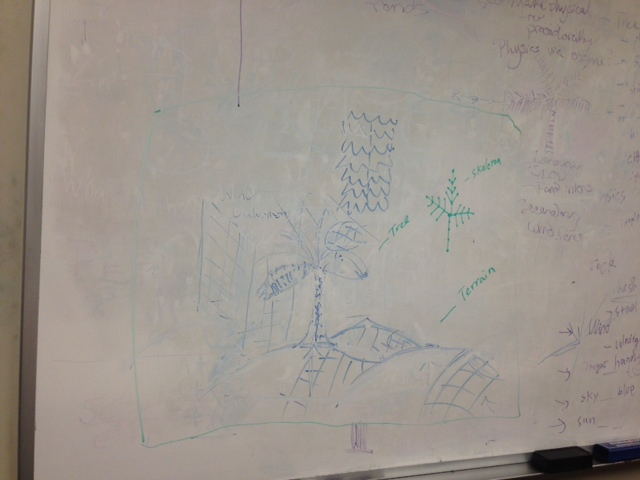
\includegraphics[height=80mm]{AbstractScene.JPG}
\caption{\textbf{Abstract Scene}}
\end{figure}

\begin{thebibliography}{11}

\bibitem{1}
GPU gems 2 : Chapter 23. Hair Animation and Rendering in the Nalu Demo by Hubert Nguyen and William Donnelly

\bibitem{2}
GPU gems 3 : Chapter 6. GPU-Generated Procedural Wind Animations for Trees by Renaldas Zioma 


\bibitem{3}
GPU gem 3: Chapter 4. Next-Generation SpeedTree Rendering by Alexander Kharlamov, Iain Cantlay and Yury Stepanenko 

\bibitem{4}
GPU gem 3: Chapter 16. Vegetation Procedural Animation and Shading in Crysis by Tiago Sousa

\bibitem{5}
Real-time Terrain Rendering using Smooth Hardware Optimized Level of Detail by Bent Dalgaard, Larsen Niels and J�rgen Christensen

\bibitem{6}
Stochastic Dynamics: Simulating the Effects of Turbulence on Flexible Structures by Jos Stam

\end{thebibliography}
\end{document}
